\documentclass{llncs}

\usepackage{url}
\usepackage{graphicx}
\usepackage{listings}
\usepackage{verbatim}
\usepackage[lined,linesnumbered,algochapter]{algorithm2e}
\usepackage{tikz}
\usetikzlibrary{arrows,automata}
\usepackage{xspace}
\usepackage{todonotes}          % Package for working draft comments
\usepackage{hyperref}           % Package for hyperlink references in the document

\usepackage[english]{babel}

\setcounter{secnumdepth}{2}
\setcounter{tocdepth}{3}

% define custom macros for specific formats or names
\newcommand{\uml}[1]{\texttt{#1}}
\newcommand{\cd}{\textsf{Class Diagram}}

\begin{document}
\pagestyle{plain}
\pagenumbering{roman}

\title{Refactoring UML models}
\author{Kristof Meixner}
\institute{\email{kristof.meixner@fatlenny.net} \\ Registration No. 9725208}

\maketitle

\begin{abstract} Over the last twenty years refactoring advanced to a commonly known and used techniques in modern
software engineering. We present an overview from the beginning of refactoring in source code to its actual application
in model-driven software development. Furthermore we discuss methods that ensure that refactored models are still
correct after modifications like static and dynamic analysis. We present research on a subset of UML that can be
executed and thus tested dynamically. At the end we introduce some works that we will adapt in our project work to
implement refactorings that are done on class diagrams and impact corresponding activity diagrams.
\end{abstract}


\tableofcontents
%\thispagestyle{plain}
\newpage

\pagenumbering{arabic}

\section{Introduction}
\label{sec:intro}

Model-based software development or model-driven software development is not only an extensive field of research but
receives also more and more attention from the industry. Nowadays models are not only used as visual explanations of
the underlying concepts but as source for the software development process itself. Thus models need to provide an abstraction of the
represented concepts in high quality. To provide quality assured software artifacts that can be used during the complete software development
life-cycle a technique called refactoring is often used to restructure in our case models. Refactorings should improve
the quality and also the understandability of the models as well as adapt the models to changes coming from the
domain. The most important requirement for refactorings is that they preserve the behavior of the model. In our project
work we focus on an set of refactorings that should be implemented taking the correlations between different model types
as well as static and dynamic analysis into account. In this work we concentrate on the related work in a broader sense
and present them in a chronological manner.

The paper is structured as follows. Section \ref{sec:beginning} copes with the early works on refactoring in the domain
of source code development. Section \ref{sec:fromto} presents how commonly known refactorings from source code where
adapted in theoretical works to models and how they can be tested for correctness with static methods. Section 
\ref{sec:todynamics} discusses actual research on how models can also be tested dynamically by executing and debugging 
the models. Finally Section \ref{sec:conclusion} summarizes the presented research.

\section{Beginning in Refactoring}
\label{sec:beginning}

In this section we will present an overview on the beginnings in structured refactoring of source code. In his thesis
Opdyke \cite{mast:REFOOF} defines refactoring as a set of operations that restructure an artifact but at the same time
preserve the behavior to increase software quality. This technique became known as refactoring.

The motivation of his work is on the one hand that software should be reused because of the high costs of development
and on the other hand that software needs to be restructured over its life-cycle to maintain this reusability. The issue
he addressed in his work is the problem of changing parts of source code from an object oriented system, grounded in a
possibly large code base while also maintaining all the references and dependencies manually. He described this a time
consuming process which is difficult and leaves room for further errors. As a solution he proposes an automated support
for refactoring which means plans to reorganize the source code on an intermediate level without changing the behavior
of the program.

A section in the thesis covers behavior preserving approaches. In this section he first mentions the usage of
\textit{preconditions} to ensure that a refactoring does not corrupt the syntax and more important does not change the
execution behavior of the program. He quickly refuses the approach to use the static compiler to test these issues as
the compiler is not capable to catch errors that change the behavior. In this section also some rules are presented that
can be tested beforehand to check if a refactoring is possible on the concepts. An important rule to mention copes with
semantic preservation of code and is described as ``Semantically Equivalent References and Operation''. He there defines
semantic equivalence such that a call of an interface with the same set of input values should result in the same set of
output values despite any change of the interals of the program. This means that from outside of a specific system
circle the refactoring is not visible. The range of this circle however differs from the impact of the refactoring on
the system. In the rest of his work he shows some examples of refactorings depending on their level of implication for
the source code for \textit{Smalltalk} program concepts and how they could be applied.

Roberts \cite{rob99}, writing his thesis at the same University, builds large parts of his contribution on the work of
Opdyke. He criticizes that the refactorings described by Opdyke are to small and can not be performed as a single
operation but often need to be done in a sequence of steps to refactor to a better ``design in mind''.  He also mentions
that the costly analysis for legal code after a refactoring should be eliminated and introduces postconditions along
with Opdykes preconditions to guarantee behavior preservation. Besides his contribution of a definition of refactoring
that also uses \textit{postconditions} Roberts presents a dependency definition of refactorings that is based on the
commutativity of single changed put in sequence. Furthermore issues an idea, which in our work seems rather interesting,
to analyze very complex refactorings not in a static manner but dynamically via refactoring during execution. This in
particular fits to our use case in the project that builds on executing and tracing changes due to refactoring before
and after the modification. Roberts also redefines the refactorings developed by Opdyke and presents his catalog that
can be used as a source for modern refactoring.

Another extensive catalog of refactorings based on source code modifications in \textit{Java} was developed and
described by Fowler in \cite{fow99}. His list of refactorings\footnote{The catalog can be found online under
http://refactoring.com/catalog/} is continuously updated and extended for different programming language and shows also
good examples how to refactor in design pattern thinking.

\section{From source code to model refactoring}
\label{sec:fromto}

In the last section we gave a brief introduction to the early research in refactoring. In this section we will discuss
what model refactoring is and how it benefit from from source code refactoring. As already mentioned in Section
\ref{sec:intro} modern software development more and more uses the concepts of model-based and model-driven approaches
which means that formal models are one of the most important artifacts in development. This also implies that changes in
the domain of the software have to be propagated to the formal models. With faster development cycles common in agile
software development like eXtreme programming (\cite{DBLP:journals/computer/Beck99}) or Scrum
(\cite{DBLP:journals/software/RisingJ00}) those changes have to be done even more efficient and reliable. It is obvious
that in this case model development benefits from the techniques of refactoring introduced in the late nineties to
source code. However models need to be treated a little different than source code.

\begin{figure}[h!t]
 \centering
 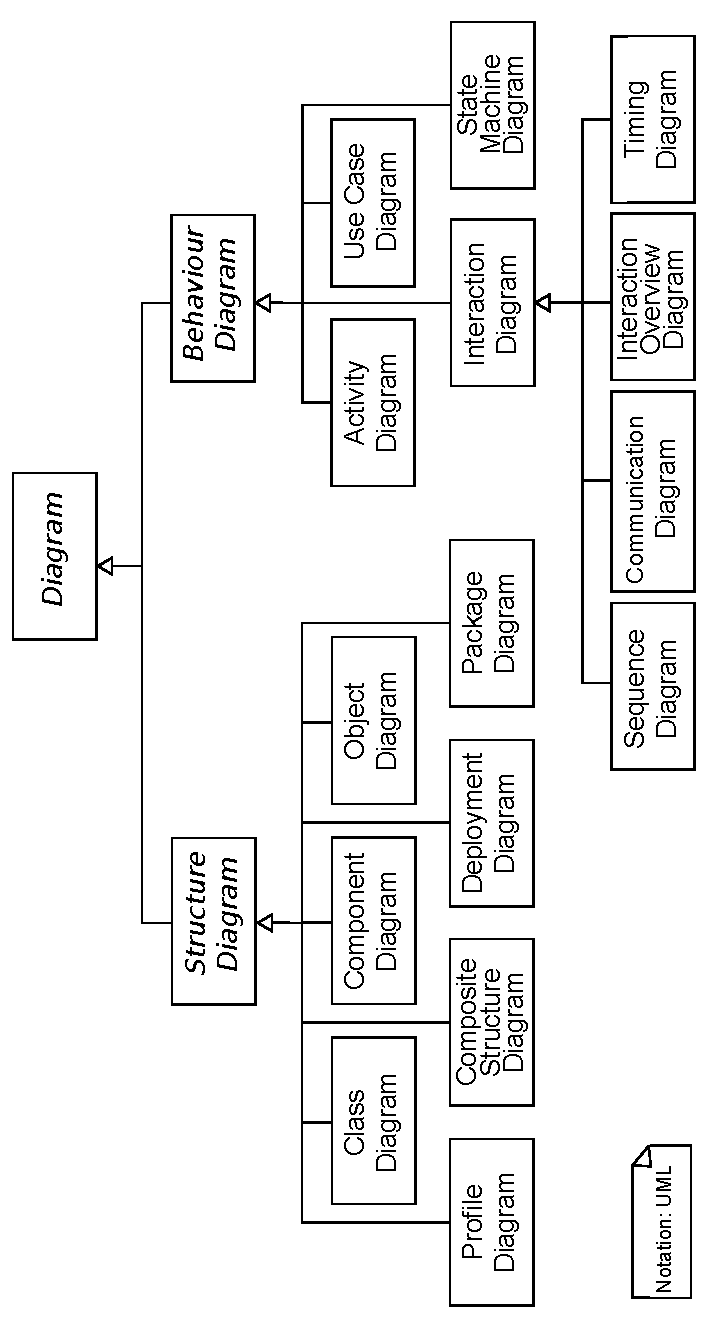
\includegraphics[scale=0.55,angle=270]{images/uml}
 \caption{\textit{UML} diagram type hierarchy (Derfel73, PMerson)}
 \label{fig:uml}
\end{figure}

Today the de-facto standard the \textit{Unified Modeling Language} (\textit{UML} - \cite{man:UML}) standardized by the
\textit{Object Management Group}\footnote{http://www.omg.org/} (\textit{OMG}) in 1997 is a general purpose language used
for model creation and development. \textit{UML} consists of an abstract syntax which builds the foundations for the
models which are formulated in the concrete syntax of the language. \textit{UML} defines several different diagram types
that can be used for designing parts of a software system. The most commonly used diagram type is the class diagram
which is often taken to depict models and components of an architecture. Generally the diagrams can be distinguished
into structural and behavioral diagrams. A further partitioning of the diagrams is shown in Figure \ref{fig:uml}. The
different diagrams share a common meta-model in the background that is often serialized in \textit{XML Metadata
Interchange}\footnote{http://www.omg.org/spec/XMI/} (\textit{XMI}) an \textit{XML} exchange format which is also
standardized by the \textit{OMG}.

The \textit{OMG} furthermore defined the \textit{Object Constraint Language} (\textit{OCL} - \cite{man:OCL}) which is a
formal language to annotate \textit{UML} models with expressions \cite{man:OCL}. The expressions specify mainly
invariants but also preconditions and postconditions that have to hold for the modeled system.

One of the first works in the domain of model refactoring was done by Suny{\'e} et al. in
\cite{DBLP:conf/uml/SunyePTJ01}. They state that refactoring of models is difficult because the impact of changes to the
model is hard to measure. This holds especially true for UML as the different model diagram types need to be taken into
account, where modeling elements often spread over views. Suny{\'e} et al. brings up an example of a class diagram and a
state chart diagram and describes how some refactorings can be applied on these models which are backed up be pre- and
postconditions formulated in \textit{OCL} to preserve the behavior of the models. The work gives a good idea how model
refactorings can be achieved and statically tested. However also the authors state that ``the search for some UML
specific refactorings has been somehow frustrating, specially when we wanted transformations to have an impact on
different UML views'' \cite{DBLP:conf/uml/SunyePTJ01}. We also somehow experienced that most of the reviewed research
concentrated only on refactoring UML class diagrams in their work.

Gorp et al. \cite{gorp03} in addition to the work before contributed a proposal for the extension of \textit{UML} in
2003 and the use of code smells in combination with \textit{OCL} pre- and postconditions to bundle so called
\textit{refactoring contracts}. Code smells are symptoms for design flaws and might indicate problems that are hidden
deeper in the source code. Gorp recommended to use a threefold process for refactoring. First use preconditions to
verify that a refactoring is possible, second use a code smell detector to find smells that indicate that the model does
not benefit from a refactoring and last but not least use the postconditions for a final check. In their research they
adapted the method for two refactorings namely \textit{pullup method} and \textit{extract method}.

Markovic and Baar in \cite{DBLP:journals/sosym/MarkovicB08} examine how refactorings of UML class diagrams impact their
corresponding OCL constraints. They presented a catalog of refactorings that leans on the catalog of Fowler and classify
them by their impact on the meta-model representation of the models. In their work they state that simple refactorings
might be easy to track and impacts may be traced and addressed on the fly, however if the meta-model representation
changes the refactorings can result in complex changes of the model and the corresponding class diagram as well as their
constraints. They therefore formalize their refactoring rules in a graphical notation included in the
\textit{QVT}\footnote{http://www.omg.org/spec/QVT/} standard by the \textit{OMG}. The grapical representation is divided
in a left hand side \textit{LHS} and a right hand side \textit{RHS}. The LHS shows the original state graph of the model
in abstract syntax and the preconditions, which have to be met such that the refactoring can be applied. The RHS shows
the state graph after the refactoring. They also present an implementation of the refactorings in
\textit{Eclipse}\footnote{http://www.eclipse.org/}.

The last research we discuss in this section is the one of Arendt and Taentzer \cite{DBLP:conf/models/ArendtTW13}.
Arendt and Taentzer relied on the work of Mohagheghi et al. \cite{DBLP:journals/infsof/MohagheghiDN09} that condensed
six classes of quality goals in model development out of several studies. Namely these are \textit{Correctness},
\textit{Completeness}, \textit{Consistency}, \textit{Comprehensibility}, \textit{Confinement} and
\textit{Changeability}. With these goals in mind they formulated a set of questions that can be checked for specific
models and show possible code smells in the underlying concepts. Furthermore they implemented a complete framework based
on the \textit{Eclipse Modeling Framework}\footnote{http://www.eclipse.org/modeling/emf/} called \textit{EMF
Refactor}\footnote{http://www.eclipse.org/emf-refactor/}. This plugin to \textit{Eclipse} allows to calculate defined
model metrics and model smells for a given model. The user can then choose from various refactorings how to improve the
model and make it more understandable. The framework can be easily extended and supports a wide range of technologies
that can be used to implement further refactorings. Besides the already mentioned build in modules \textit{OCL}
additional modules can be created in \textit{Java}, \textit{Henshin}\footnote{https://www.eclipse.org/henshin/} a
transformation engine for \textit{EMF} and \textit{ComRel} ``a model-based language for the combination of EMF model
refactorings''.

\section{From static to dynamic testing}
\label{sec:todynamics}

In the section above we presented some works that cover refactoring of models and use different methods of static
analysis to ensure that the behavior of the models are preserved and to identify models that where not well designed. In
this section we will discuss research that adapts the approach presented by \cite{rob99} and uses the execution of
systems to dynamically verify the behavior of models.

\textit{UML} does not provide the semantics to make a model as executable as program code is. This issue was issued in
the definition of a subset of textit{UML} that narrows the semantics of the concepts down to make them executable. This
subset is defined in the standard ``Semantics of a Foundational Subset for Executable UML Models'' (textit{fUML} -
\cite{man:FUML}). If you recall Figure ref{fig:uml} textit{fUML} supports two diagram types, the class diagram and the
activity diagram. The class diagram can be used to model the domain with its concepts, the activity diagram can be used
to describe the behavior of the concepts in the class diagram. The abstract syntax of textit{fUML} differs slightly
from the one of textit{UML}.

\begin{figure}[h!t]
 \centering
 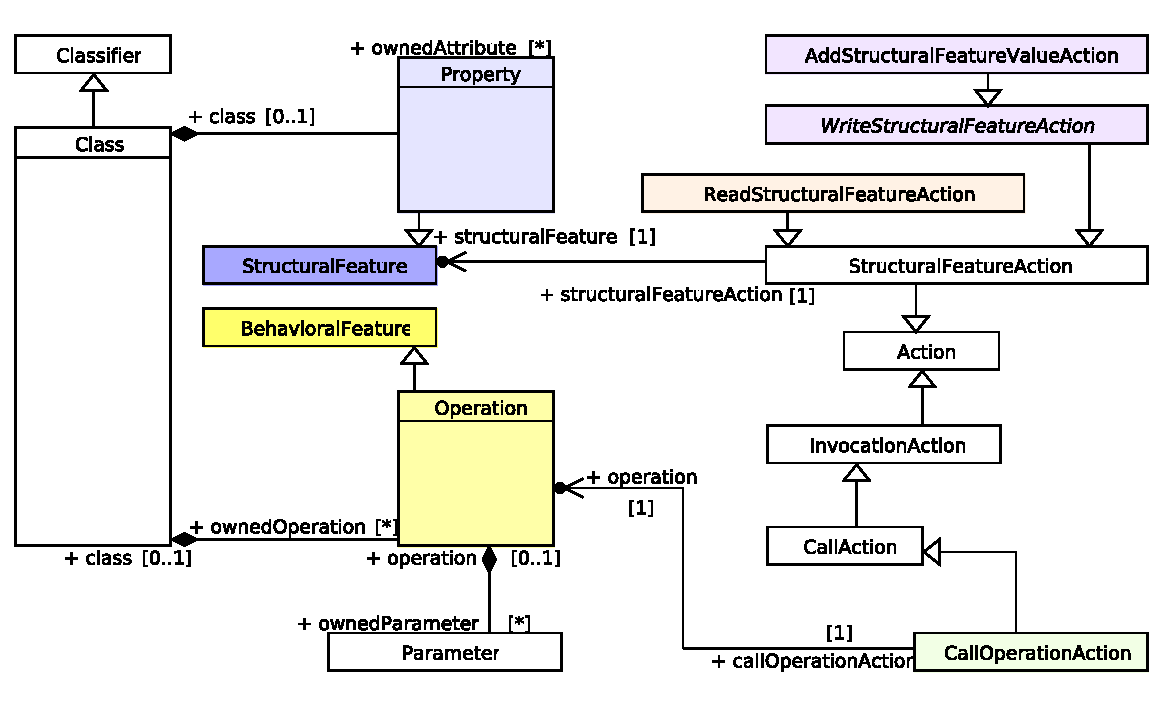
\includegraphics[scale=0.9]{images/Model_Model_Classifiers}
 \caption{Abstract syntax for used class concepts in \textit{fUML}}
 \label{fig:fuml1}
\end{figure}

\begin{figure}[h!t]
 \centering
 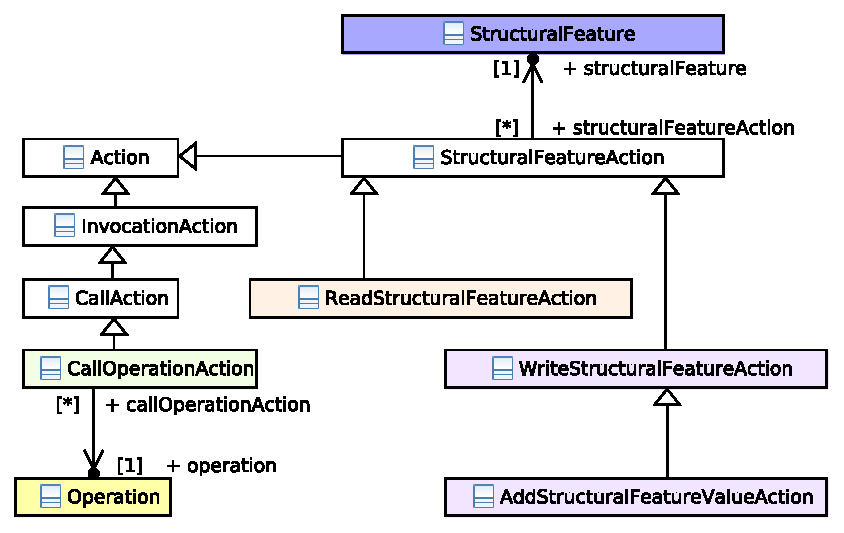
\includegraphics[scale=0.9]{images/Model_Model_Behavior}
 \caption{Abstract syntax for used actions in \textit{fUML}}
 \label{fig:fuml2}
\end{figure}

In our project work we concentrate on this subset to investigate the changes that are implied in the corresponding
diagram if the other diagram changes. For this work we only apply refactorings on the class diagram and observe the
changes implied in the activity diagram as this to be the more reasonable use case. In order for the reader to get more
insight on the topic we provide a simple \textit{encapsulate field} example refactoring. The refactoring has the
following steps:

\begin{itemize}
 \item Create setters and getters for the attribute.
 \item Change all occurrences of the attribute to the created setters and getters.
 \item Change the attribute to private.
\end{itemize}

In Figure \ref{fig:fuml1} and \ref{fig:fuml2} the abstract classes for the class diagram and the activity diagram are
displayed. For the class diagram there are nearly no modifications except to create the new methods and set the
attribute to private. In an activity diagram it is not that obvious. Figure \ref{fig:calculatePremiumRef} shows a very
simple activity diagram. Each of the actions \lstinline|readNumberOfVehicles|, \lstinline|readCustomer| and
\lstinline|readAge| read \lstinline|StructuralFeatures| shown in violet in the figures are actions of type
\lstinline|StructuralFeatureAction|. Each of these actions have to be changed to \lstinline|CallOperationActions| as the
accessed parts of the class diagram changed to operations shown in turquoise. In this simple model it seems rather easy
but in complex models dependencies grow and make necessary changes it hard to target.

\begin{figure}[h!t]
 \centering
 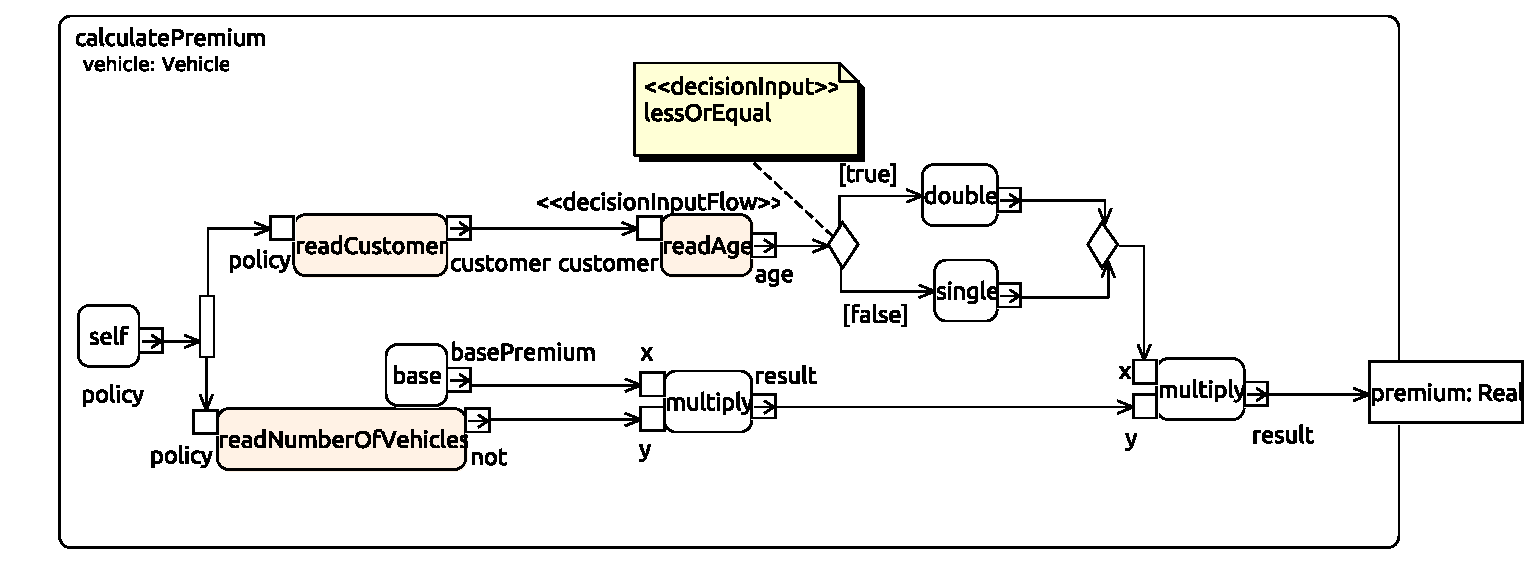
\includegraphics[scale=0.5]{images/insurance_ref/Activity_calculatePremium_calculatePremium}
 \caption{Calculate premium activity diagram with refactorings}
 \label{fig:calculatePremiumRef}
\end{figure}

Mayerhofer proposes in \cite{DBLP:conf/icse/Mayerhofer12} to use common techniques from software development to
dynamically verify the behavior of refactored models namely testing and debugging. However some problems come up when
taking a deeper look because ``UML models constitute a multiple view specification of a system''. In a further
scientific work by Mayerhofer et al. \cite{DBLP:conf/models/MayerhoferLK12} a runtime model is presented that is capable
to execute and trace activities. They also implemented\footnote{http://www.modelexecution.org/} a virtual machine that
is capable of running \textit{fUML} models and can even convert \textit{UML} model compatible to \textit{fUML} for
execution purposes.

For our project work we use this reference work to implement a set of refactorings test the pre- and postconditions on
them and run them in the virtual machine after refactoring to verify the preservation of their initial behavior.

\section{Conclusion}
\label{sec:conclusion}

We presented a brief overview on the scientific work in the domain of refactoring over the last twenty years. It ranges
from simple source code refactoring with pre- and postconditions and developed to the domain of model-driven development
where refactoring is equally needed but harder to implement because of the different views on the underlying models and
their correlations. Model development tries to take common techniques from source code development and adapt them for
its needs. While from the beginning static analysis was taken into account in the later research and especially with the
standardization of \textit{fUML} also dynamic analysis like testing and debugging during execution is introduced.

For our project work we are going to use a combined approach and use static as well as dynamic model testing to
implement a set of refactorings for class and activity diagrams.

\newpage
\bibliographystyle{acm}
\bibliography{references}

\end{document}
